 % intro
\documentclass[../main.tex]{subfiles}

\begin{document}

\subsection{Symbols Index} 
Unless stated otherwise, the following notation will be used:
\begin{itemize}
    \item $\C$, complex plane
    \item $\widehat{\C}$, Riemann sphere.
    \item $\partial E$, boundary of $E$
    \item $\overline{E}$, topological closure of $E$
    \item $f$, analytic function of a complex variable.
    \item $\mathcal{O}(z)$, orbit of $z$
    \item $z^*$, fixed point of $f$ assumed to be 0  without further specification
    \item $\nhd \subseteq \C$, neighbourhood of the fixed point $z^*$.
    \item $\lambda=f'(z^*)$, first term in the power series expansion of $f$.
    \item $\iter{f}{n}$, $n$-fold iterate of $f$
    \item $p \in \Z_{\geq 1}$, the smallest integer for which the coefficient of $z^{p+1}$ term in the power series of $f$ is non-zero.
    \item $\D_{r} = \left\{z \in \C \mid \abs{z} < r \right\}$. We often write $\D = \D_{1}$
    \item $\R/\Z$, the circle group consisting of \emph{angles} viewed as the interval $[0, 1)$
    \item $\fatou(f)$, the Fatou set of $f$ 
    \item $\julia(f)$, the Julia set of $f$
    \item $\basin_{f}(z^*)$, basin of attraction of $z^*$ for the function $f$. If it is obvious what $f$ is, we simply write $\basin(z^*)$
    \item $\basin^0(z^*)$, immediate basin of attraction of $z^*$
    \item $\basin^{0}(\mathcal{O}, f)$, immediate basin of periodic orbit
    \item $\mathrm{Log}$, the principal logarithm
    \item $\kulia{(f)}$, the filled Julia set of $f$
    %% add anything else 
\end{itemize}

\newpage
\section{Introduction and motivation}
\label{sec:intro}

Let $f : \nhd \tendsto \C$ be a complex function analytic in some set $\nhd \subseteq \C$. Suppose further that $z^* \in \nhd$ is a fixed point of $f$, $f(z^*) = z^*$ and consider the so-called \emph{forward orbit} of $z \in \nhd$
\[
\mathcal{O}(z) := \left\{z, f(z), \iter{f}{2}(z), \dots, \iter{f}{n}(z), \dots \right\}
\]
(which may be finite or infinite), where
\[
\iter{f}{n} = \underbrace{f \circ f \circ \dots f \circ f}_\text{$n$}
\]
is the $n$-fold iterate of $f$ so long as this is defined on $\nhd$. A natural question is what behaviour can we expect for a given $z \in \nhd$. This question, and more generally the dynamics of this system, have been extensively studied across the twentieth and twenty first century as can be seen in (Cremer 1938), (Siegel 1942), (Milnor 2006) or (Buff and Ch\'eritat 2012). In this work, we will primarily be occupied with understanding local behaviour of such a holomorphic function $f$ around a fixed point $z^*$. To this end, notions of \emph{normalisation} will be of particular interest, namely in allowing us to classify and determine the dynamics of the above system without having to directly compute iterations of $f$.

We will often work in $\C$ but at places also consider the Riemann sphere $\widehat{\C} = \C \cup \{\infty\}$. We also assume elementary results from complex analysis and topology. The definition of the Riemann sphere along with certain results can be found in the appendix. 

\begin{exl}\label{ex 1.1}
Suppose $f(z) = \frac{2z^3+1}{3z^2}$. We have fixed points at $\fix = 1, e^{2\pi i/3}, e^{4\pi i/3} $ . Then even small perturbations to the initial condition cause changes in behaviour; 
\begin{align*}
  \lim_{n \rightarrow \infty} \iter{f}{n}(0.4i) &= e^{4\pi i/3}\\
  \lim_{n \rightarrow \infty} \iter{f}{n}(0.42i) &= e^{2\pi i/3} \\
\lim_{n \rightarrow \infty} \iter{f}{n}(0.415i) &= 1  
\end{align*}
\end{exl}

This motivates the idea of classifying the dynamical behaviour of an analytic function $f$ so as to determine which regions of the complex plane correspond to what behaviour and construct \emph{normal forms} to classify functions that display certain dynamics. For the above example, see Figure \eqref{fig:Julia of example}.

We first consider a way of dividing the plane into regions that correspond to \emph{sensitive dependence on the initial condition}. That is, points where small perturbations can result in wildly different behaviour.

\begin{dfn}
    \label{intro:dfn:fj}
    A family of holomorphic functions $F$ is called \emph{normal} on some domain $\Omega \subseteq \C$ if every sequence of functions in $F$ has a subsequence that is \emph{locally uniformly convergent} on $\Omega$. That is, every sequence in $F$ has a subsequence that converges uniformly on compact subsets $K \subseteq \Omega$.
\end{dfn}

\begin{dfn}
    For an analytic function $f:\nhd \to \C$, the \emph{Fatou set} of $f$, denoted $\fatou(f)$, is the largest set on
    which the family of iterates $\left\{\iter{f}{n}\right\}$ is normal. The \emph{Julia set}, denoted $\julia(f)$, is the complement of the Fatou set, $\julia(f) = \C\setminus\fatou(f)$
\end{dfn}

Here, $z_0 \in \julia(f) \Longleftrightarrow$ in a neighbourhood of $z_0$, there is the aforementioned sensitive dependence on the initial point.

\begin{figure}
    \label{fig:Julia of example}
    \centering
    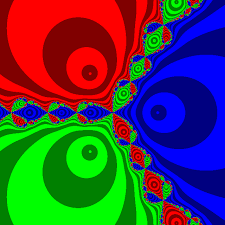
\includegraphics[width=6cm]{resources/ch-11/Juliaex.png}
    \caption{Regions of the complex plane corresponding to initial conditions that converge to one of the three fixed points. Here, $\julia(f)$ is the shared boundary consisting of the half-lines $\arg{z} = \pi, \pi/3, 5\pi/3$ and indeed contains $0.4i$ (Geyer 2016).}
\end{figure}

\begin{dfn}
\begin{enumerate}
    \item Let $g, h$ be analytic functions. We say $g$ is \emph{conjugate} to $h$ if there exists a local biholomorphic map $\phi$ such that
    \[
    \phi \circ g \circ \phi^{-1} = h
    \]
    \item With $f : \nhd \to \C$ as above, the \emph{multiplier} of a fixed point $\fix$ is defined as $\lambda := f^{\prime}(\fix)$
    \item A point $z \in \nhd$ is a \emph{periodic point with period $q$} of $f$ if $\iter{f}{q}(z) = z$ and $\iter{f}{(q+1)}(z) \neq z$
\end{enumerate}
\end{dfn}

It is clear that conjugacy is an equivalence relation and the equivalence classes are called \emph{conjugacy classes}. A key property is that the dynamics of our system are preserved under conjugation, more specifically the multiplier $\lambda$ is independent of the choice of coordinate chart.

\begin{lem}
Let $g = \phi \circ f \circ \phi^{-1}$ be conjugate to $f$. Then
\begin{enumerate}
    \item $\fix$ is a fixed point of $f \Longleftrightarrow \phi(\fix)$ is a fixed point of $g$
    \item $z$ is a $q-$periodic point of $f \Longleftrightarrow \phi(z)$ is a $q-$periodic point of $g$
    \item If $\fix$ is a fixed point of $f$ with multiplier $\lambda$, then $\phi(\fix)$ is a fixed point of $g$ with multiplier $\lambda$
\end{enumerate}
\end{lem}
\begin{proof}
\begin{enumerate}
    \item $\phi(\fix)$ is a fixed point of $g \Longleftrightarrow \phi(f(\fix)) = \phi(\fix) \Longleftrightarrow f(\fix) = \fix$. Hence we have a bijection $\phi$ from the set of fixed points of $f$ to that of $g$
    \item It is clear that $\iter{g}{q} = \phi \circ \iter{f}{q} \circ \phi^{-1}$. If $z$ is $q-$periodic, then $z$ is a fixed point of $\iter{f}{q}$ so $\phi(z)$ is a fixed point of $\iter{g}{q}$ by $(1)$. If $\iter{g}{(q+1)}(\phi(z)) = \phi(z)$, then $\phi(\iter{f}{(q+1)}(z)) = \phi(z) \Longrightarrow \iter{f}{(q+1)}(z) = z$ which contradicts the definition of $z$ being $q-$periodic. The converse holds by a similar argument.
    \item This immediately holds by the chain rule since 
    \begin{align*}
        g^{\prime}(\phi(\fix)) &= (\phi \circ f \circ \phi^{-1})^{\prime}(\phi(\fix)))\\
        &= (\phi\inv)^{\prime}(\phi(\fix))\phi^{\prime}(f(\fix))f^{\prime}(\fix)\\
        &= f^{\prime}(\fix) = \lambda
    \end{align*}
    \end{enumerate}
\end{proof}

Since the dynamics of $f$ are preserved under conjugation, if $\fix$ is a fixed point of $f$, we can assume without loss of generality that $\fix = 0$ by conjugating $f$ by a M\"obius transformation that carries $\fix \longmapsto 0$. Thus, henceforth unless stated otherwise, we study the behaviour of iterating the analytic function
\begin{equation}
    \label{intro:eq:f}
    f(z)= \lambda z + a_2 z^2 + a_{3} z^3 \dots
\end{equation}
in some neighbourhood $\nhd$ of the origin.


Specifically, we will come to see that the multiplier $\lambda=f'(0)$ dictates the local behaviour of $f$ above corresponding to the following cases:
\begin{enumerate}
    \item \emph{Geometrically Attracting or Repelling}:
    $\abs{\lambda}\notin \{0, 1\}$
    \item \emph{Superattracting}: $\lambda = 0$
    \item \emph{Parabolic}: $\lambda=e^{2\pi i\xi}$ for rational $\xi$
    \item \emph{Irrationally Indifferent}: $\lambda=e^{2\pi i\xi}$ for irrational $\xi$
\end{enumerate}
    
A further classification arises from considering the equivalence relation of conjugacy. As we have seen in a small sense, conjugate maps have qualitatively similar dynamics. With this we hope to find \emph{normal forms} of $f$, that is simple maps that are conjugate to $f$, which not only classify the local behaviour of $f$ but also allow us to conclude such dynamics without arduous computation. Finding such normal forms will be a key objective of each following chapter.
\end{document}
